\todopar{Discuss the Mephisto laser head. Laser basics. Non-planar
ring oscillator. Beam shape. Frequency and intensity noise.
}
We start with a Mephisto 2 Watt laser head with an integrated intensity
noise reduction system.
This laser has good noise characteristics on its own.
It is a \ac{ndyag} \ac{npro} laser. The monolithic cavity allows for an
extemely small spectral linewidth of less than 1kHz \ac{fwhm}. The noise
eater option gives a \ac{rin} of less than -150dB/Hz.
It's lasing medium is one solid piece of \ac{ndyag} with four internally reflecting
surfaces that form a ring shaped cavity. Three points define a plane, the
addition of the fourth mirror outside of this plane enables a rotation of
the polarization of the laser for each round trip around the ring. With the addition
of a permanent magnet, there will be a Faraday rotation as well which is
dependant on the direction of the laser around the ring. For one direction
the polarization rotation from the two effects are cancelled. In the other
direction, the polarization rotations are not cancelled and light leaks out
of the cavity at a rate higher than the gain of the medium due to a slight
polarization dependent reflection of the input mirror. The output beam ends
up with a very narrow linewidth but a slight elliptical shape.

Although the laser has a very good noise performance, we wish to clean it up
even further in certain regions of interest. We have assembled three systems
for this. The first is an \ac{iss} which provides active feedback to the laser
intensity. Then there is the \ac{fss} which provides active feedback to the
frequency. There is also a \ac{pmc} which is also an active feedback system. The
\ac{pmc} is used in conjunction with the \ac{iss} to ensure that we are
sensing the zero order Gaussian mode of the laser because this is what
we will ultimately be coupling into the trap cavity.

\section{Intensity Stabilization}
\todopar{Paragraph on the theory of operation}

% The \ac{iss} is a genuinely eccentric animal with long, pointy ears and a fluffy
% tail. It allows us to see things with incredible accuity. Far better than
% previous generations of furniture.\footnote{Silly rambling, it happens...}

The \ac{iss} uses a \ac{pd} for sensing the laser power from a pick-off
beam after the \ac{pmc}. This gives us sensing of the amount of power in
the TEM00 mode of the laser we are using for our experiment. The signal is
fed back through an electronic servo to an actuator that modulates the
intensity of the beam before the \ac{pmc}. The actuator is an \ac{aom}.

\subsection{Sensing}
\todopar{Photo-electric effect, quantum efficiency}

The \ac{pd} works by the photoelectric effect. There is a quantum
efficiency associated with each \ac{pd} which is the amount of light quanta
(photons) which are converted into electrical current.
\begin{align}
q.e. &= \frac{N_{el}}{N_{ph}} \\
     &= \frac{I/e}{P/(\hbar \omega)} \\
     &= \frac{2 \pi \hbar c}{e \lambda} \frac{I}{P} ,
\end{align}
where $e$ is the elementary charge.

This relates the
power of the incident light to the current in the output of the \ac{pd}.
Photodiode quantum efficiency is usually specified in Amps per Watt.
This must naturally be dependent on the wavelength of the light, so they must
also specify a wavelength.

We are limited by noise due to counting statistics (shot noise). We want a high signal
to noise. In this case, the signal that we are concerned about is the
relative fluction in power, and so it is proportional to the DC incident
power on the \ac{pd}. The noise, as a Poissonian process, is proportional
to the square root of the DC power (or the number of photons per second).

The \ac{rin} becomes the photon counting error divided by the total number
of photons.
\begin{align}
\mathrm{RIN} &= \frac{\sqrt{N_{el}}}{N_{el}} \\
     &= \frac{1}{\sqrt{N_{el}}} \\
     &= \frac{1}{\sqrt{q.e. \times N_{ph}}} \\
     &= \sqrt{\frac{\hbar \omega}{q.e. \times P \tau}} \, ,
\end{align}
where $\tau$ is the integration time. This allows us to write the amplitude
spectral density of the shot noise in $\mathrm{RIN} / \sqrt{H\!z}$ as,
\begin{align}
\sqrt{\frac{2 \hbar \omega}{q.e. \times P}} \, ,
\end{align}
where the 2 is due to the choice of one-sided spectra.

\subsection{Feedback}
\todopar{Electronics}

The electronics were designed to reduce intensity noise above about 4 Hz to
about 1kHz or so. It is in this region where the experiment takes place.

\subsection{Actuation}
\todo{Description of Acousto-Optic Modulator}

Actuation, as mentioned above, is accomplished using an \ac{aom}. The
\ac{aom} is a device which can modulate a laser beam in both frequency
and intensity. It works by using bragg reflections in a crystal with
travelling waves. The interaction between the travelling waves and crystal
lattice divert the beam to different orders of refraction. The power in each
order is dependant on primarily the amplitude of the travelling waves. The
diffraction angle is dependant on the wavelength of the travelling waves.
We take the zero order refraction and modulate on the intensity of the
waves which, in turn, modulated the amount of power diverted into higher order
Bragg refractions.

\section{Frequency Stabilization}

The \ac{fss} is an active feedback system which stabilizes the already quite
narrow frequency from the laser. The system is composed of a rigid laser cavity
which is used as a reference which we can lock the laser frequency to. The
laser frequency follows the length of the reference cavity up to several kHz.

\subsection{Sensing}

Sensing for the \ac{fss} is accomplished using the method of \ac{pdh}.
(see \cite{Black:2001})
The signal is essentially the derivative of the reflected power with respect
to frequency of the laser (assuming length is fixed).
This is accomplished by modulating the frequency of the input beam with an
\ac{eom} driven by a 25MHz local oscillator and demodulating the reflected
beam with the same local oscillator.
%This measures the relative amplitude of the reflected light as opposed to the
%amplitude squared (power).
The result is a signal on resonance that is zero and has maximum slope
(see fig.\ref{fig:pdh}).
Exactly the signal we want for a feedback system which keeps the laser on
resonance with the cavity. 

\begin{figure}
\centering
\tikzsetnextfilename{pdhplot}
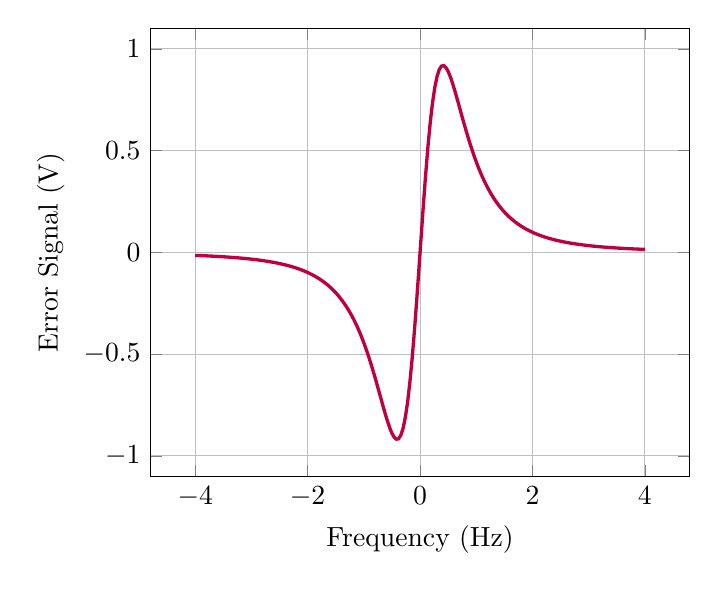
\begin{tikzpicture}
\begin{axis}[
    samples=200,
    grid=both,
    xlabel={Frequency $(\mathrm{Hz})$},
    ylabel={Error Signal $(\mathrm{V})$}
    ]
%  \addplot[blue,domain=-4:4,very thick] {x*exp(-x*x)};
  \addplot[purple,domain=-4:4,very thick] {x/(x*x+0.5)/(x*x+0.5)};
\end{axis}
\end{tikzpicture}
\caption[PDH Error Signal]{This shows the \ac{pdh} error signal. Our lock point
  must be between the positive and negative cavity poles (maximum  and minimum on
  the y-axis).
  }
\label{fig:pdh}
\end{figure}

\subsubsection{Cavity Assembly}

The reference cavity is a Fabry Perot made from an 8 inch monolithic fused silica
spacer with high reflectivity mirrors glued onto the ends. The reflectivity
of the mirrors yield a finesse of about 7600. Finesse is defined as the ratio
of the \ac{fsr} to the cavity linewidth (\ac{fwhm}). One can arrive the
relationships between FSR, Finesse, mirror reflectivity as follows,
\begin{align}
E_{\mathrm{cavity}} =& E_{\mathrm{incident}} \sqrt{1-r_1^2} \left( 1 + r_1 r_2
    e^{i \omega 2 L /c} + \left(1+r_1 r_2 e^{i \omega 2L/c} \right)^2 + \ldots \right)
    \\
=& E_{\mathrm{incident}} \sqrt{1-r_1^2} \left( \frac{1}{1 - r_1 r_2
    e^{i \omega 2L/c}} \right)
\end{align}
Now, we find the reflected field,
\begin{align}
E_{\mathrm{reflected}} =& E_{\mathrm{incident}} \left( 1-r_1^2 \right)
    \left( \frac{r_2 e^{i \omega 2L/c}}{1 - r_1 r_2 e^{i \omega 2L/c}} \right)
    - r_1 E_{\mathrm{incident}}
\end{align}

\subsubsection{Cavity Suspension}
\begin{figure}[htbp]
	\centering
		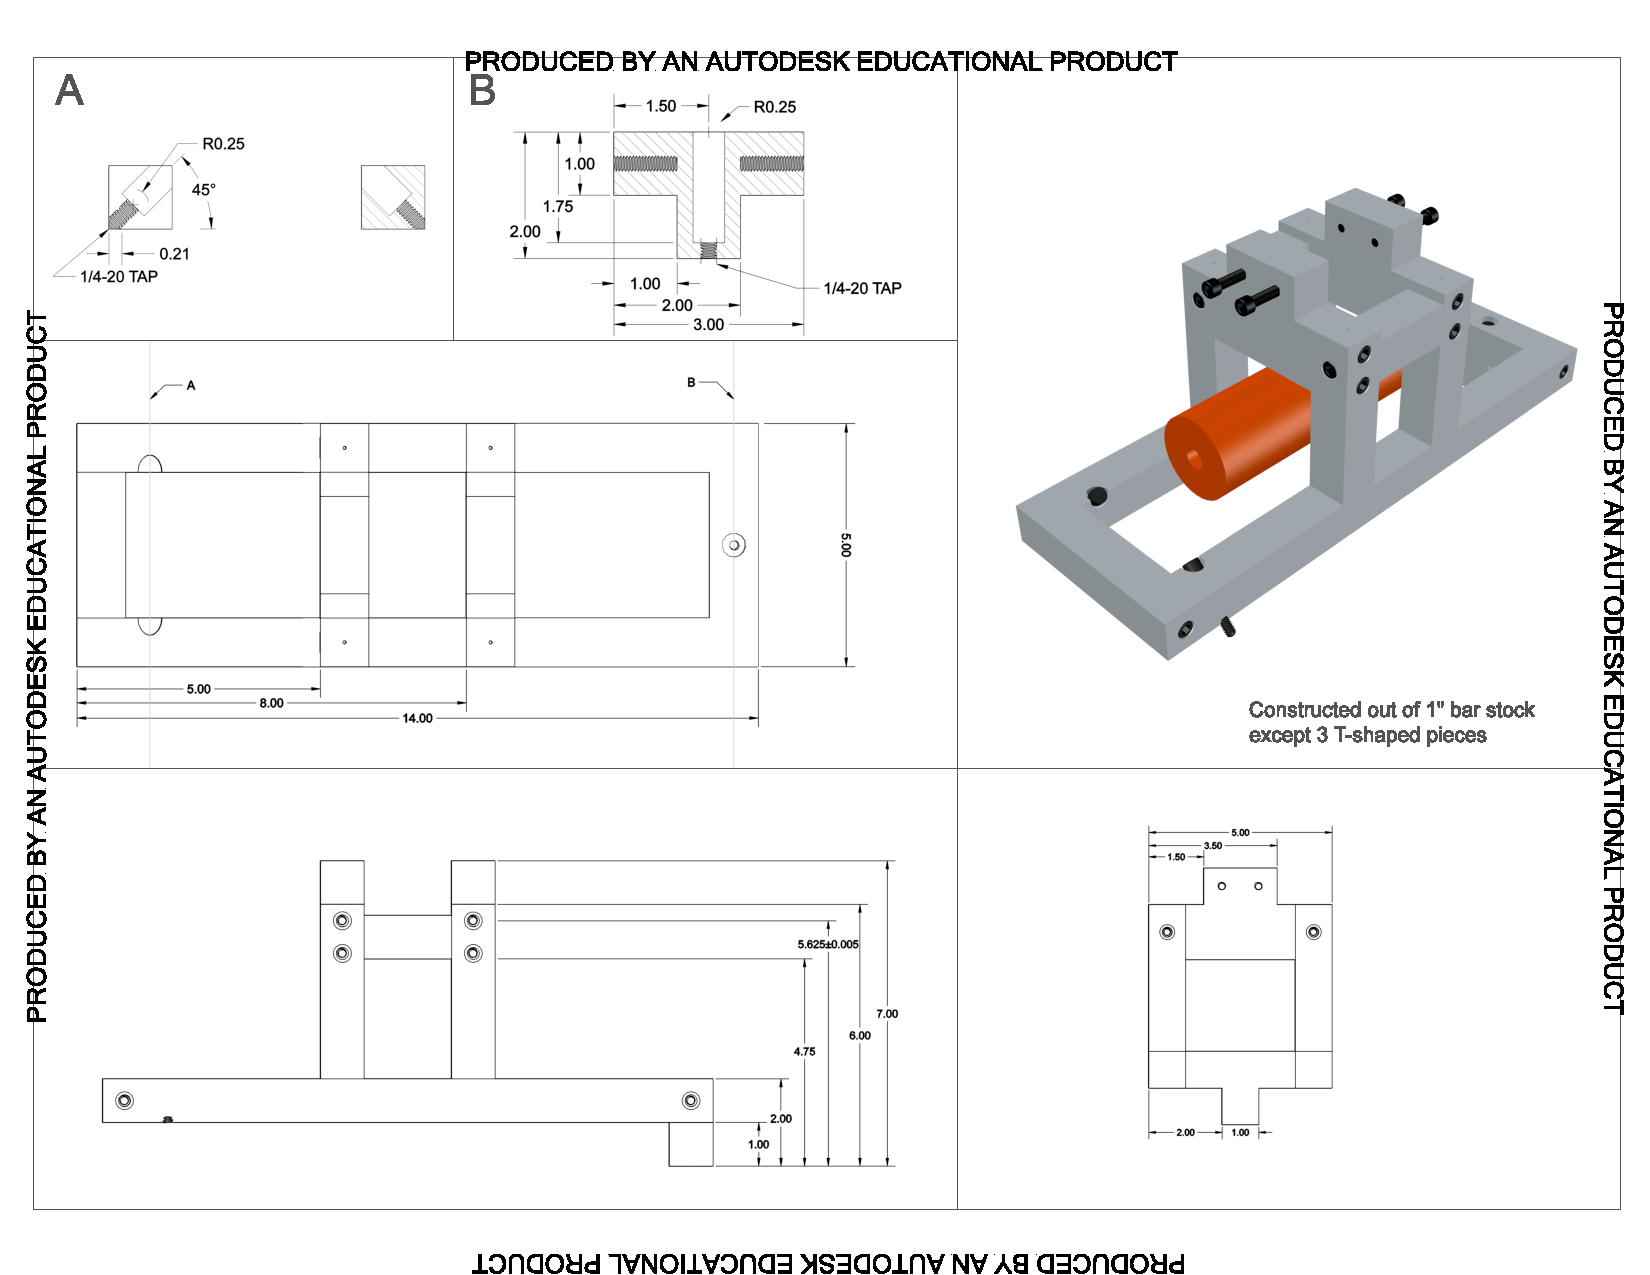
\includegraphics[width=15cm]{./figures/refcavsusdesign.pdf}
	\caption[Reference Cavity Suspension Design]{Design of the reference cavity suspension}
	\label{fig:refcav_sus}
\end{figure}

\subsubsection{PDH Locking}

\subsection{Feedback}
The feedback electronics used for the \ac{fss} are from initial LIGO. The board
provides feedback signal for 2 different actuation paths. The low frequency path
is to the laser cavity length which is split again into two different actuation
paths (thermal control and a piezo electric transducer in the laser head). The
other path is to an \ac{eom} to actuate on the phase of the laser beam.

\subsection{Actuation}

There are three actuators. Low frequency actuation is by a thermal controller in
the laser head which actuates on the the cavity length through thermal expansion.
The mid frequency actuation is by \ac{pzt} which applies a force to change the
cavity length. The high frequency actuation is by phase modulation of the light
after it exits the laser head using an \ac{eom}.

%\todopar{Add a description of the Electro-Optic Modulator}

%\subsubsection{Laser Head Thermal}
%
%\subsubsection{Laser Head Piezo-Electric Transducer}
%\todopar{add description of peizo-electric effect}
%\todopar{describe the effects of the piezo in-loop}

\subsubsection{Electro Optic Modulator}

\section{Mode Cleaner}
%\todopar{add description of PMC, reference Willke,98}
The PMC is a ring cavity of three mirrors.
see  \cite{Willke:98}


\subsection{Sensing}

\subsection{Feedback}

\subsection{Actuation}
Actuation on cavity length is done with a piezo-electric transducer on one of
the mirrors. This transducer converts voltage to cavity length.

